\documentclass[20pt,a4paper]{report}
\usepackage[T2A,T1]{fontenc}
\usepackage[utf8]{inputenc}
\usepackage{blindtext}
\usepackage[russian]{babel}
\usepackage{mwe}
\usepackage{graphbox}
\usepackage[document]{ragged2e}
\usepackage[margin=50pt]{geometry}
\usepackage{longtable}
\usepackage{fontspec}
\usepackage{float}
\usepackage{titlesec}
\usepackage{setspace}
\usepackage{minted}

\usepackage{hyperref}
\hypersetup{
    colorlinks,
    citecolor=black,
    filecolor=black,
    linkcolor=black,
    urlcolor=black
}

\setstretch{1.5}
\graphicspath{{./images/}}
\setmainfont{LiberationSerif}
\setmonofont{Hack}
\titleformat{\chapter}{\normalfont\LARGE\bfseries}{\thechapter}{1em}{}
\titleclass{\chapter}{straight}
\titlespacing{\chapter}{0pt}{0pt}{5pt}[25pt]


\begin{document}
	\begin{titlepage}
		\begin{minipage}{0.3\textwidth}
		
\includegraphics[scale=0.03]{logo.png}	
		\end{minipage}
		\begin{minipage}{0.6\textwidth}\centering
			\textbf{
				Министерство науки и высшего образования Российской Федерации
				Федеральное государственное бюджетное образовательное 
				учреждение высшего образования
				«Московский государственный технический университет
				имени Н.Э. Баумана (национальный исследовательский университет)»
				(МГТУ им. Н.Э. Баумана)
			}	
		\end{minipage}
	
		\vspace{5cm}
		\centering
		\Large
		\textbf{
			Лабораторная работа №8 \\
			по курсу «Разработка интернет-приложений» \\
		}

		\vspace{6cm}
		\begin{flushright}
			Выполнил \\ 
			студент группы ИУ5-54Б \\ 
			Сысойкин Е.М. 
		\end{flushright}
		\vspace{5cm}
		Москва, 2020
	\end{titlepage}

	\chapter{Описание задания}
	\large
	\begin{enumerate}
		\item Создайте прототип веб-приложения с использованием фреймворка Django: \\
		\begin{itemize}
			\item Создайте виртуальное окружение.
			\item Установите в него Django.
			\item Создайте проект и приложение Django.
		\end{itemize}
		\item Создайте представления и шаблоны (по желанию можно использовать модели), реализующие концепцию master/detail со следующей функциональностью: \\
		\begin{itemize}
			\item На странице master в виде списка HTML выводится информация о трех объектах (например, о трех сортах мороженого). Каждая строка списка представляет собой гиперссылку, при нажатии на которую происходит переход к странице detail.
			\item Страница detail содержит детальное описание объекта (сорта мороженого), фотографию, гиперссылку на master-страницу.
			\item Фотография относится к статическому содержимому сайта.
			\item Страница detail должна выводить данные с использованием таблицы HTML.
			\item Шаблон страницы detail получает от представления данные о детальном объекте с использованием контекста.
			\item НЕОБЯЗАТЕЛЬНЫЙ ПУНКТ. По желанию можно использовать верстку с применением Bootstrap (или аналогичного фреймворка), а также представления на основе классов (class-based views).
		\end{itemize}
	\end{enumerate}
	
	\chapter{Текст программы}
		\qquad \textbf{myapp/fill\_data.sql} \\
		\small
		\inputminted[tabsize=4, linenos, breaklines]{sql}{myapp/fill_data.sql}
		\large
		
		\qquad \textbf{myapp/myapp/urls.py} \\
		\small
		\inputminted[tabsize=4, linenos, breaklines]{python}{myapp/myapp/urls.py}
		\large
		
		\qquad \textbf{myapp/myapp/apps.py} \\
		\small
		\inputminted[tabsize=4, linenos, breaklines]{python}{myapp/myapp/apps.py}
		\large
		
		\qquad \textbf{myapp/myapp/views.py} \\
		\small
		\inputminted[tabsize=4, linenos, breaklines]{python}{myapp/myapp/views.py}
		\large
		
		\qquad \textbf{myapp/myapp/models.py} \\
		\small
		\inputminted[tabsize=4, linenos, breaklines]{python}{myapp/myapp/models.py}
		\large
		
		\qquad \textbf{myapp/myapp/templates/master.html} \\
		\small
		\inputminted[tabsize=4, linenos, breaklines]{html}{myapp/myapp/templates/master.html}
		\large
		
		\qquad \textbf{myapp/myapp/templates/detail.html} \\
		\small
		\inputminted[tabsize=4, linenos, breaklines]{html}{myapp/myapp/templates/detail.html}
		\large
		
	\chapter{Экранные формы}
		\begin{figure}[H]
			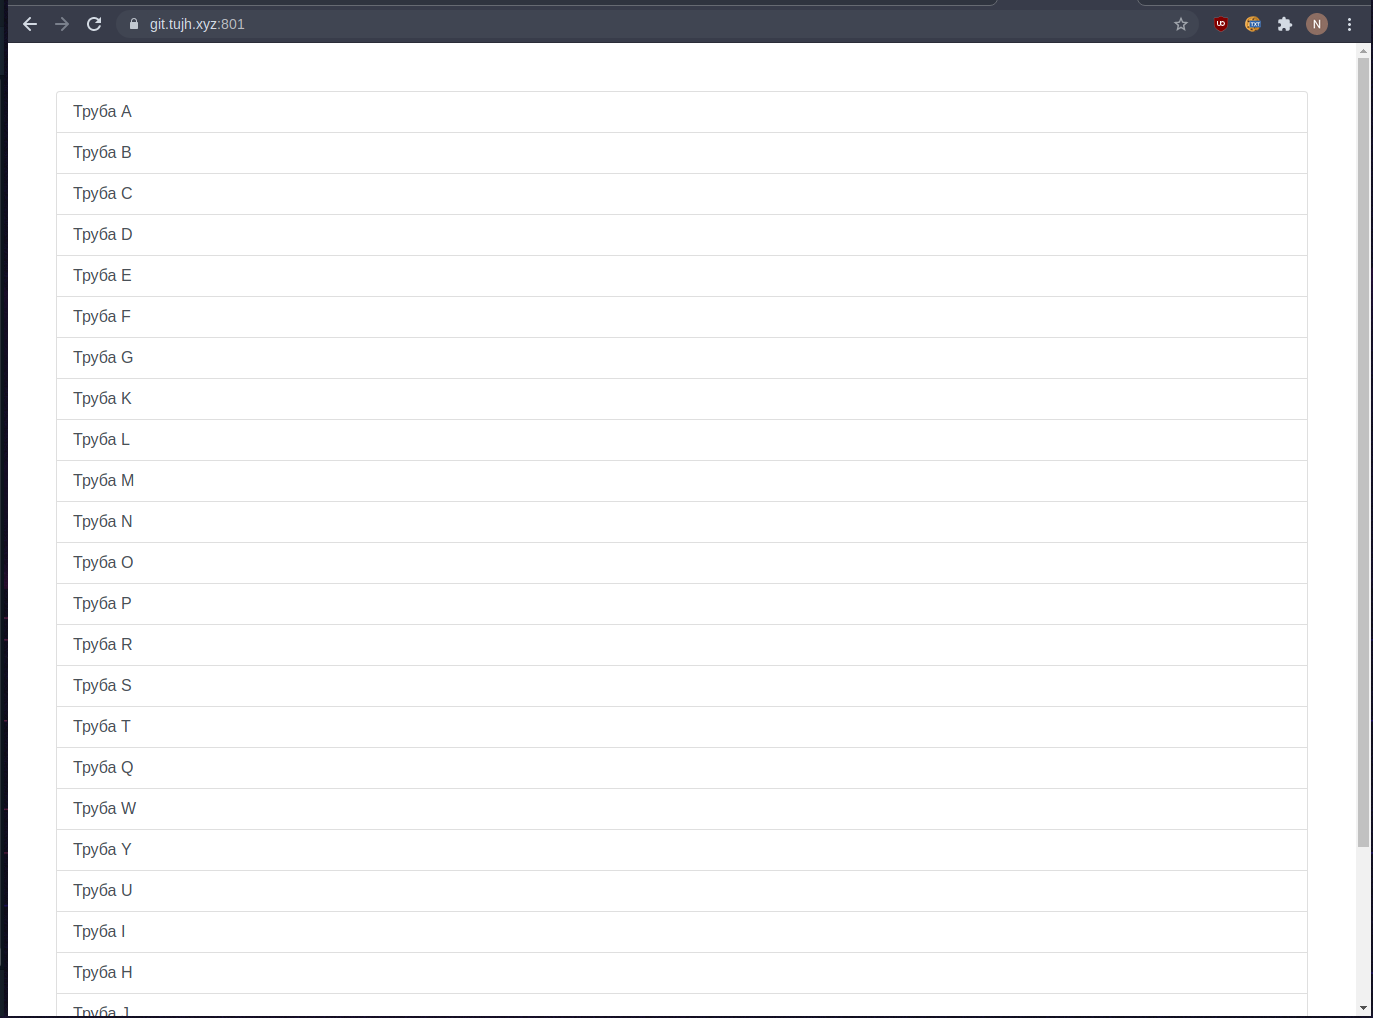
\includegraphics[width=\textwidth]{1.png}
		\end{figure}
		\begin{figure}[H]
			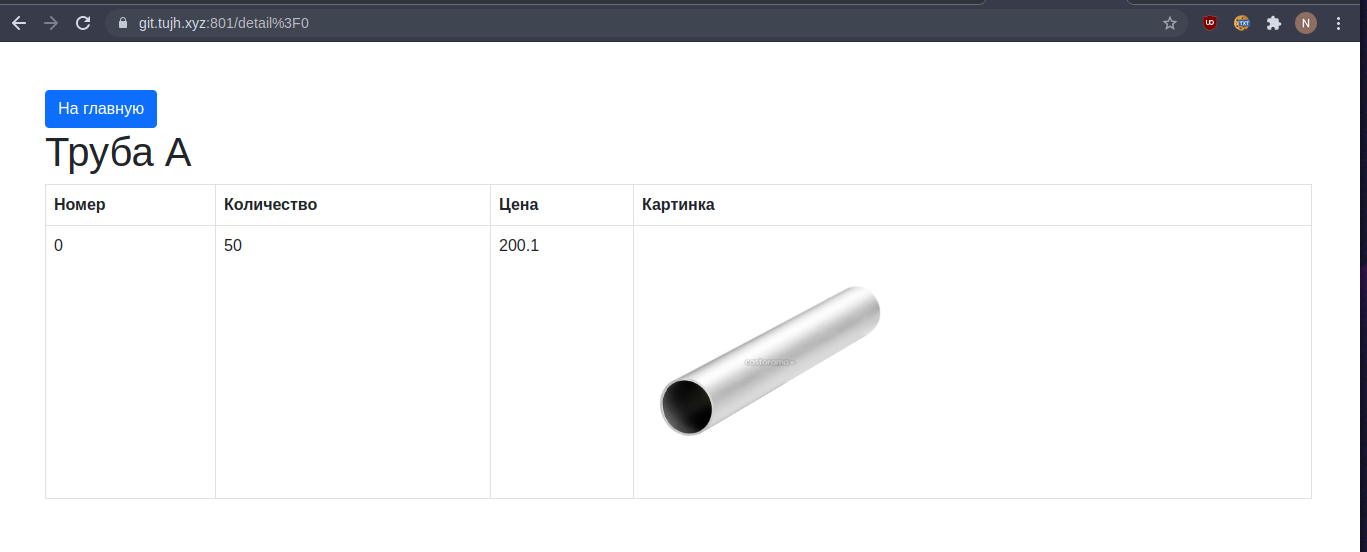
\includegraphics[width=\textwidth]{2.png}
		\end{figure}

\end{document}

